\documentclass[11pt]{article}
\usepackage{enumerate}
\usepackage{tikz,tikz-cd,tikz-3dplot,pgfplots}
\usepackage{amsmath,amsthm,amssymb,amsfonts,amsthm}
\usepackage{mathrsfs}
\usepackage{bm,bbm}
\usepackage{braket}
\usepackage{slashed}
\usepackage{tensor}
\usepackage{indentfirst}
\usepackage[a4paper, total={6.5in, 9in}]{geometry}
\usetikzlibrary{decorations.markings,positioning,decorations.pathmorphing}
\allowdisplaybreaks
\pgfplotsset{width=10cm, compat=1.16}
\renewcommand\bra[1]{{\langle{#1}|}}
\renewcommand\ket[1]{{|{#1}\rangle}}
\renewcommand\bfdefault{b}

\newtheorem{theorem}{Theorem}[section]
\newtheorem{lemma}[theorem]{Lemma}
\newtheorem{corollary}{Corollary}[theorem]
\theoremstyle{definition}
\newtheorem{definition}{Definition}[section]
\theoremstyle{remark}
\newtheorem{remark}{Remark}[section]

\DeclareMathOperator{\sech}{sech}
\DeclareMathOperator{\csch}{csch}
\DeclareMathOperator{\arcsec}{arcsec}
\DeclareMathOperator{\arccot}{arccot}
\DeclareMathOperator{\arccsc}{arccsc}
\DeclareMathOperator{\arccosh}{arccosh}
\DeclareMathOperator{\arcsinh}{arcsinh}
\DeclareMathOperator{\arctanh}{arctanh}
\DeclareMathOperator{\arcsech}{arcsech}
\DeclareMathOperator{\arccsch}{arccsch}
\DeclareMathOperator{\arccoth}{arccoth} 

\begin{document}
	metric convention: $(+,-,-,-)$
	
	Lagrangian:
	\[\mathcal{L}=\frac{1}{2}\partial_{\mu}\phi\partial^{\mu}\phi-\frac{1}{2}M^{2}\phi^{2}+\partial_{\mu}\chi^{\dagger}\partial^{\mu}\chi-m^{2}\chi^{\dagger}\chi-g_{3}\phi\chi^{\dagger}\chi-g_{4}\phi^{2}\chi^{\dagger}\chi.\]
	
	\section{Diagram 1}
	\begin{center}
		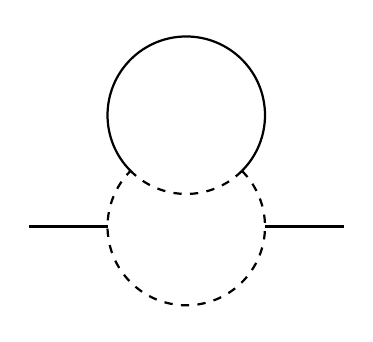
\begin{tikzpicture}[thick]
			\tikzstyle{every node}=[font=\large]
			\def\len{1cm}
			\draw (-2*\len,0) -- (-\len,0);
			\draw (2*\len,0) -- (\len,0);
			\draw[dashed] ({sqrt(0.5)*\len},{sqrt(0.5)*\len}) arc (45:-225:\len);
			\draw[dashed] ({sqrt(0.5)*\len},{sqrt(0.5)*\len}) arc (-45:-135:\len);
			\draw ({sqrt(0.5)*\len},{sqrt(0.5)*\len}) arc (-45:225:\len);
		\end{tikzpicture}
	\end{center}
	\[\Pi_{1}(p^{2})=g_{3}^{4}\int\frac{d^{d}q}{(2\pi)^{d}}\frac{d^{d}r}{(2\pi)^{d}}\left(\frac{1}{q^{2}-m^{2}}\right)^{2}\frac{1}{r^{2}-m^{2}}\frac{1}{(p-q)^{2}-m^{2}}\frac{1}{(q-r)^{2}-M^{2}}.\]
	First loop evaluation ($r$):
	\begin{align*}
		\Pi_{1}(p^{2})&=g_{3}^{4}\int\frac{d^{d}q}{(2\pi)^{d}}\left(\frac{1}{q^{2}-m^{2}}\right)^{2}\frac{1}{(p-q)^{2}-m^{2}}\int\frac{d^{d}r}{(2\pi)^{d}}\frac{1}{r^{2}-m^{2}}\frac{1}{(q-r)^{2}-M^{2}}\\
		&=:g_{3}^{4}\int\frac{d^{d}q}{(2\pi)^{d}}\left(\frac{1}{q^{2}-m^{2}}\right)^{2}\frac{1}{(p-q)^{2}-m^{2}}P_{1}.
	\end{align*}
	\begin{align*}
		P_{1}&=\int dx\int\frac{d^{d}r}{(2\pi)^{d}}\Big((1-x)(r^{2}-m^{2})+x[(q-r)^{2}-M^{2}]\Big)^{-2}\\
		&=\int dx\int\frac{d^{d}r}{(2\pi)^{d}}\Big((r-xq)^{2}-x^{2}q^{2}-(1-x)m^{2}+xq^{2}-xM^{2}\Big)^{-2}\\
		&=\int_{0}^{1}dx\int\frac{d^{d}k}{(2\pi)^{d}}\Big(k^{2}-\Delta_{1}\Big)^{-2}\\
		&=\frac{i}{(4\pi)^{2-\epsilon}}\Gamma(\epsilon)\int_{0}^{1}dx\,\frac{1}{\Delta_{1}^{\epsilon}},
	\end{align*}
	where $l=r-xq$ and $\Delta_{1}=-x(1-x)q^{2}+(1-x)m^{2}+xM^{2}$.
	
	The integrand can be rewritten as following:
	\begin{align*}
		&\left(\frac{1}{q^{2}-m^{2}}\right)^{2}\frac{1}{r^{2}-m^{2}}\frac{1}{(p-q)^{2}-m^{2}}\frac{1}{(q-r)^{2}-M^{2}}\\
		&=24\int dF_{4}\,x\Big(x(q^{2}-m^{2})+y(r^{2}-m^{2})+z[(p-q)^{2}-m^{2}]+w[(q-r)^{2}-M^{2}]\Big)^{-5}
	\end{align*}
	where $\int dF_{4}=\int_{0}^{1}dx\,dy\,dz\,dw\,\delta(x+y+z+w-1)$.
	
	\section{Diagram 2}
	\begin{center}
		\begin{tikzpicture}[thick]
			\tikzstyle{every node}=[font=\large]
			\def\len{1cm}
			\draw (-2*\len,0) -- (-\len,0);
			\draw (2*\len,0) -- (\len,0);
			\draw[dashed] (0,0) circle (\len);
			\draw (-0.2*\len,0.8*\len) -- (0.2*\len,1.2*\len);
			\draw (-0.2*\len,1.2*\len) -- (0.2*\len,0.8*\len);
		\end{tikzpicture}
	\end{center}
	
	\section{Diagram 3}
	\begin{center}
		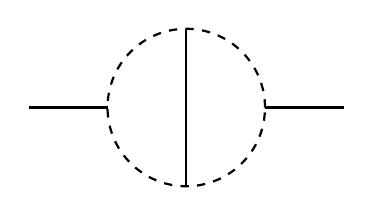
\begin{tikzpicture}[thick]
			\tikzstyle{every node}=[font=\large]
			\def\len{1cm}
			\draw (-2*\len,0) -- (-\len,0);
			\draw (2*\len,0) -- (\len,0);
			\draw[dashed] (0,0) circle (\len);
			\draw (0,-\len) -- (0,\len);
		\end{tikzpicture}
	\end{center}
\end{document}